\documentclass[12pt,a4paper]{article}

% --- Essential Packages ---
\usepackage[utf8]{inputenc}
\usepackage[T1]{fontenc}
\usepackage{graphicx}    % For Orange screenshots
\usepackage{booktabs}    % For professional tables
\usepackage{amsmath}     % For math/accuracy formulas
\usepackage{geometry}    % For 1-inch margins
\usepackage{xcolor}      % For colored text
\usepackage{titlesec}    % For clean section headings
\usepackage{hyperref}    % For clickable TOC and links
\usepackage[framemethod=TikZ]{mdframed} % For highlighted key points
\usepackage{xcolor}
\usepackage{parskip} % for better spacing between paragraphs
\usepackage{caption} % For better control over figure captions
\usepackage{float} % For precise figure placement

% Define the box style
\mdfdefinestyle{takeawaybox}{
    roundcorner=5pt,
    linecolor=gray!50,
    backgroundcolor=gray!5pt,
    innertopmargin=10pt,
    innerbottommargin=10pt,
    innerleftmargin=10pt,
    innerrightmargin=10pt
}
\geometry{margin=1in}
\hypersetup{colorlinks=true, linkcolor=blue, urlcolor=cyan}

% --- Document Metadata ---
\title{
    \Huge \textbf{Driver Drowsiness Detector} \\
    \vspace{0.5em}
    \Large Hardware Project Evaluation
}
\author{
    \textbf{Charles Smelt} \\
    \small F331073
    }
\date{\today}

\begin{document}

\maketitle

\newpage
\tableofcontents
\newpage

\section{Introduction}
The aim of this project is to create a versatile piece of hardware that can be used to improve road safety.
With use of a Raspberry Pi 4B and a camera (I have opted for a web cam as they are cheap and wildly accessible),
I will be aiming to produce a light weight AI based system to detect a drivers tiredness and aim to either wake
them up, warn them of their condition or even potentially come up with a viable solution. I will further aim to
inform the driver through use of a wireless digital display. For this, I am aiming to use the users own WIFI
enabled device to connect to the Pi and broadcast data, warning as and other information. Since this will be
presented to the user via a web page, I would further like the user to be able to interact with the system to
Taylor it to themselves and their set up, to get the best function out of the project.

\subsection{Why Do This?}
Many accidents on the road are caused by drivers lack attention due to dreariness. With ‘10-20\%’ [1] of all
crashes on the road believed to have been attributed to tiredness; one in four fatalities estimated to have had
tiredness play a part on UK roads, this is a serious problem. Not only this but given that an incident occurs on
UK roads ‘Every 17 minutes’ [2] where ‘someone is killed or seriously injured’ [2], something needs to change. 

\section{Research}
\subsection{Tiredness Identifiers}
There are several different ways to identify tiredness, especially when driving. Somes examples are:
\begin{itemize}
    \item More frequent blinking – this is because your eyes and brain function to counter fatigue and discomfort
    \item Harder Blinking – prolonged opening can result in them being saw and dry, so, to combat this, your body
    makes you blink harder and more frequently to keep them lubricated
    \item Delayed reaction times – neurons in your brain slow as they process information less efficiently
    \item Your head can begin to drop as you inevitably slowly fall asleep (worst case)
    \item Yawning – this is your body’s attempt to both keep your brain awake as well as cool the body
    \item Grip loosens – your body begins to relax as you fall asleep, actions aren’t made with the same intent
    \item Mood changes – you can often become more irritable as you fall asleep
    \item Snoring – if you have already fallen asleep, you relax and this can result in snoring
\end{itemize}

\subsection{Driving Effected Factors}
As you get more tired, you often lose concentration. You can’t find yourself reacting more slowly and your decision
making can become impaired. You can also become a more violent or unstable driver as your mood can be easily influenced
as you do not have the energy to combat how you feel. Not only this, but in the worst case (int eh event of falling
asleep) you can no longer operate the vehicle.

\subsection{Legality of Using a Mobile Device}
In this project, I would like to make use of the users’ own device, which will probably be their mobile phone. To get
around the legal issue of using a mobile device, it will have to be securely fastened in a cradle and not held by the
driver. Furthermore, I will not be able to request interaction from the driver once the vehicle is in motion unless I
use hands-free \cite{gov_mobile_law}, "for example:
\begin{itemize}
    \item A Bluetooth headset
    \item Voice commands
    \item A dashboard holder or mat
    \item A windscreen mount
    \item A built-in satnav” 
\end{itemize}
Failure to comply with this can result in 6 penalty points and a £200 fine. But this can go up to a driving ban as
well as a maximum of £1000 fine.

\begin{mdframed}
\textbf{Key Implementation Takeaways:}
\begin{itemize}
    \item \textbf{Setup Protocol:} User-interactive features must be restricted to the initial setup phase while the
    vehicle is stationary.
    \item \textbf{Motion Safety:} Integration of the device's internal accelerometer to disable interactive displays
    during motion, ensuring the system does not become a distraction.
\end{itemize}
\end{mdframed}

\subsection{Potential Models and Algorithms}
\subsubsection{Initial thought process – basic Convolutional Neural Netwrk (CNN):}
My initial idea was to follow a methodology I had previously learnt in one of my prior modules, using a simple
Convolutional model consisting of input nodes containing extracted values from an image, and then train the model to
detect these trends in data to predict an outcome. For this I made use of Mediapipe’s face mesh to extract features from
frames extracted from videos, to form inputs into the neural network. This was my initial thought process, and with a desire
to start coding, and deliver a prototype, I naively started to develop this without additional research.

This was methodology and implementation is talked about in ‘Simple AI Models’ section of this document. Here I explain my
methodology and thought process (as well as data validation) as to why I believed this method feasible in the early stages of
this project.

Following this failure, which is also expressed in the ‘Simple AI Models’ section I expanded my research to other AI models which
will follow.

\subsubsection{Deep Convolutional Models:}
As an expansion from the idea above, this consists of a far greater number of layers. With its main uses in image identification,
this would be ideal for the task at hand. One key difference being the number of layers. This adds size and complexity to the
network, which may make it more difficult to run on the Pi compared to other models due to its increased parameter size as a result
of its increases in width and levels.

\subsubsection{Xception Model (Extreme Inception):}
A development of the normal inception model, this stands as the middle ground between regular convolutional models and depthwise
separable convolutional models (depthwise + pointwise). This makes better use of parameters than the Inception v3  model rather than
reducing the number of parameters. This is done through channel mixing.

By removing the multi branch capabilities of an inception model, opting for a single branch this completely decouple spatial
correlations as well as branch correlations, which results in more focused learning .

To take this further, you can make use of pre-trained models. The example I have used in the Inception Models section of this
paper was trained on the ImageNet dataset. This transferred learning allows for pre-learns identification of edges, shapes and facial
structure to be applied to my current data, without the need for the network to necessarily learn these itself, rather re-enforce its
previous learning with my new data. This should allow for a model which learns faster, requiring less time to train, as well as a more
accurate model, due to its additional pre-training.
Some information gathered from \cite{xception}.

\subsubsection{CondenseNet:}
This is an example of an “Efficient DenseNet using Learned Group Convolutions”[10]. This was designed for mobile use, with the aim of
requiring limited computational power by removing connections between layers, aiming to remove redundancies which are not used in the
later layers. Due to this, only one tenth of the computation is required compared to the DenseNet (a Deep Convolutional Model where all
layers are connected to every other layer, rather than one layer being connected to the next). Comparable to MobileNet (an Inception
model approach which focuses on efficiency and power usage rather than accuracy) but requiring less computation.
This is done through pruning in the early stages of learning to form a ‘sweet spot’ \cite{condensenet} in between sparsity and
regularity. Essentially,group (cluster) sizes are reduced (e.g. $3 \times 3 \to 1 \times 1$) which results in less computation, but a
loss in accuracy, and requirement of more grouping of inputs.
The idea of this is to reduce the number of connections during learning, to improve computational speeds and re-enforce routes, at the
cost of accuracy. 

\subsubsection{Further Development Ideas / Key Takeaways:}
\paragraph{Model Selection}
On such a small number of classifications and training examples for each classification, CondenseNet may not be the best option for
this project. While it is said to be faster and more optimizable for a device with limited computational ability and power (like the
Raspberry Pi I am using), it requires a greater quantity of training data than I have, without crossing between sources, and for the
sake of this project, I believe that this may be beyond the scope of what is required for success – but this may change as the project
progresses.
Xception, while slower, can provide greater accuracy given the training data that I have. This would be good for experimenting on what
the greatest achievable accuracy of a model given my training data could be. Not only this, but this model is available in Tflite, so
it is possible for the performance to be improved while on the Pi. While not necessary, this is a nice bonus and something worth
considering.
Documentation on this can be found at \url{https://keras.io/api/applications/xception/}.

\paragraph{Pre-train Options:}
To improve the versatility of these AI models, the images that are used for training should be altered to allow for a more versatile
classification. 
Since users will be using this at day and night, it would be beneficial to alter some of the training data (if it isn’t already at
day and night) by adjusting the \textbf{brightness} to simulate darkness or lower light conditions such as changes in cloud cover or
going through a tunnel.  \textit{(±15°)}

The camera angle and position can also change depending on how the user sets up the system. While the location of the recordings
cannot be changed in post, the \textbf{angle} can. This will help to provide some fixability in the model, to still allow for detection
of tiredness, even if the set-up is not perpendicular to the driver, like in most of the recordings.  \textit{(±20\%)}

Another issue is \textbf{zoom}. My hardware, as well as the hardware between the different training data sources, is different. As a
result, my inputs may automatically be different based on camera zoom, and how the user positions their face in the focus region,
so fluctuations in zoom/crop may be a thing to consider.  (0.9 $\to$ 1.1 zoom/crop)

\subsubsection{Information Communication:}
\paragraph{Webpage Hosting}
With this project being done in python, for ease of use and versatility of existing libraries for the AI section of this project, it
would be best to utilize some existing python libraries for the webpage.

\subparagraph{Flask and Alternate Frameworks}
Flask is a lightweight web framework used for web-based interfaces and API’s. In the case of this project, it would be used to host
the local webpage. This will allow for offline communication of the drowsiness state. 

Tkinter and PyQt provide a graphical use interface (idea for what I need), however, have a far more limited flexibility as well as
requiring a physically connected device which will further limit how the project will function and be operated as additional wiring
will create clutter as the user does not use something which id found in the vehicle anyway. As a result, neither of these frameworks
are likely to be considered in the final result.

Django is a very powerful framework, however, with this comes complexity for a system with such simple routing and visualization
requirements.

Another example of another framework to consider is REACT. With past experience in other projects, this has the upside that I understand
it already. However, with the project being aimed to be as light as possible to improve efficiency, this client-heavy framework might
not be the best for this project.

Overall, the low resource requirements and lightweight nature of this project, as well as the majority of the code base being in
python, the obvious choice seems to be Flask to provide a platform-independent web interface.

\subparagraph{API}
A simple way of connecting the webpage to the AI model. There are several different ways of communicating data from the tiredness
detection AI to the webpage:
\begin{itemize}
    \item \textbf{Shared File:} The idea is that both programs for AI detection and web hosting are run simultaneously with a common
    file to relay information between them. However, this could be more compute heavy, something I have expressed repeatedly as being
    something I want to reduce. Additionally, this can result in race conditions, where there is inconsistency between the file and the
    actual value. From a hardware point of view, with files being stored on the SD card (with limited numbers of writes) this method
    can result in shortfalls in the long run.
    \item \textbf{Shared Database:} Using some form of database (e.g. SQLite) can provide additional information as well as filtering.
    However, because of the simplistic nature of this project, it is likely too costly to do this. While given more time, and a greater
    fixation on tracking and suggested improvements to inform the user of patterns or issues, this is not in the scope of this project. 
    \item \textbf{Use of integrated API:} This is the least expensive option in terms of computing power. You can make use of threading
    to keep the two lightweight, related programs, together. This makes it easier to manage and in the event of failure of the AI, the
    whole program knows (as opposed to being in the dark due to each program being separate).
\end{itemize}

Therefore, Option 3 (combined server and AI runner with threading) was selected as it minimizes computational overhead, avoids disk I/O
bottlenecks, and keeps the architecture simple for this real-time detection application. 





\newpage
\section{Plan}
In this section, I will outline a brief outline of my intended plan of action, which will likely be reformed later on as other issues
become more present during the development process.

\subsection{Time Management:}
\begin{figure}[h]
    \centering
    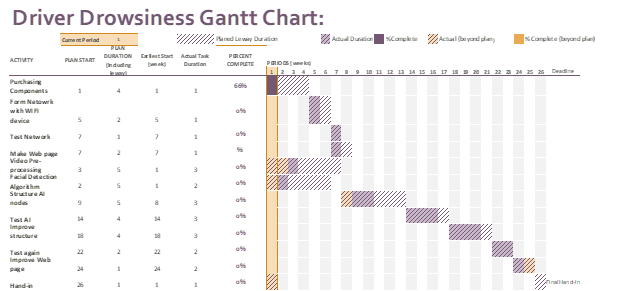
\includegraphics[width=0.9\textwidth]{Images/Gantt_chart.png}
\end{figure}

Here week one refers to the starting week (w/c 20.10.2025) and week 26 being the week of the deadline (w/c 20.04.2025).
The initial delay in this project is due to shipping of components. Since I do not have any of the components that I need to do this
project, I will have to order them, and this takes time. However, in the meantime, I can request permission for datasets as well as
gather a better understanding of what attributes can affect a driver’s concentration and different potential models that I could use for
my lightweight AI component.

\subsection{Connections:}
Since raspberry pie 4 is WIFI compatible, I plan to connect the user’s own device by this. Therefore, using the pi as a host device for
a website that can display data and other information to the user. This is the ideal option as wired displays either require the pi to be:
\begin{itemize}
    \item Dashboard mounted due to a small wire. This has the potential to fall or move, causing further irritation or distraction for
    the driver. This is against the aim of the project of keeping the driver focused on the road.
    \item More wires and additional screens for setting up. Once again, this takes up space in their field of vision and will create
    added hassle if setting up for different drivers. Most people will likely opt to not use this device, making it a futile construction.
\end{itemize}
By using the users’ own wireless device, you not only remove the added expense of the screen (if released to the commercial market) but
also remove clutter. Users are likely to already have phone mounts in their desired location, so why not give the idle device some added
functionality. This will also be optional, if they are already using the device for maps, it will not prevent the system from relaying
information or alerting the user.

\begin{figure}[H]
    \centering
    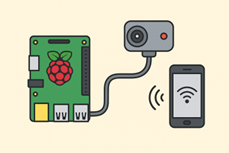
\includegraphics[width=0.7\textwidth]{Images/pie_idea.png}
    \captionsetup{labelformat=empty}
    \caption{\tiny (ChatGPT generated –> prompt=”please make this look nice + drawing of this”)}
\end{figure}






\newpage
% RREFERENCES
\begin{thebibliography}{99}

\bibitem{brake_fatigue}
Brake. (2026). ``Driver Fatigue Knowledge Centre.'' \url{https://www.brake.org.uk/get-involved/take-action/mybrake/knowledge-centre/driver-fatigue}

\bibitem{road_safety}
Brake. (2026). ``UK Road Safety Knowledge Centre.'' \url{https://www.brake.org.uk/get-involved/take-action/mybrake/knowledge-centre/uk-road-safety}

\bibitem{SUST}
Kavalci Yilmaz, E., and Akcayol, M. A. (2022). ``SUST-DDD: A Real-Drive Dataset for Driver Drowsiness Detection.'' \textit{Proceedings of the 31st FRUCT Conference}, 31:416--21. doi: 10.5281/zenodo.6519933.

\bibitem{ortega2020dmd}
Ortega, J. D., et al. (2020). ``DMD: A Large-Scale Multi-modal Driver Monitoring Dataset for Attention and Alertness Analysis.'' \textit{Computer Vision — ECCV 2020 Workshops}, pp. 387--405. Springer International Publishing.

\bibitem{yang2023fatigueview}
Yang, C., Yang, Z., Li, W., and See, J. (2023). ``FatigueView: A Multi-Camera Video Dataset for Vision-Based Drowsiness Detection.'' \textit{IEEE Transactions on Intelligent Transportation Systems}, vol. 24, no. 1, pp. 233--246. doi: 10.1109/TITS.2022.3216017.

\bibitem{gov_mobile_law}
UK Government. (2024). ``Using a mobile phone while driving.'' \url{https://www.gov.uk/using-mobile-phones-when-driving-the-law}

\bibitem{BINA}
Isworo, N., and Liawatimena, S. (2025). ``Annotated Drowsiness Detection Dataset Captured Using Raspberry Pi 5.'' \textit{Mendeley Data}, V1. doi: 10.17632/chvz7vh2dc.1

\bibitem{convolutional}
Szegedy, C., et al. (2015). ``Going deeper with convolutions.'' \textit{2015 IEEE Conference on Computer Vision and Pattern Recognition (CVPR)}, pp. 1--9.

\bibitem{xception}
Chollet, F. (2017). ``Xception: Deep Learning with Depthwise Separable Convolutions.'' \textit{2017 IEEE Conference on Computer Vision and Pattern Recognition (CVPR)}, pp. 1800--1807.

\bibitem{condensenet}
Huang, G., et al. (2018). ``CondenseNet: An Efficient DenseNet Using Learned Group Convolutions.'' \textit{2018 IEEE/CVF Conference on Computer Vision and Pattern Recognition}, pp. 2752--2761.

\end{thebibliography}  
\end{document}